\subsection{Interrelación Pregunta - Alumno Curso Académico}

   \begin{description}
      \item[Definición] En esta interrelación se deja constancia de que un
      determinado alumno recibe preguntas, por parte de su asesor, que deberá
      responder.

      \item[Características] La interrelación presenta las siguientes
                             características:

         \begin{itemize}
            \item \textbf{Nombre:} P-AlCA
            \item \textbf{Tipo de la interrelación:} Fuerte.
            \item \textbf{Cardinalidad de la interrelación:} N:M
                  \begin{itemize}
                     \item Pregunta: formulada\_a (0,n)
                     \item Alumno Curso Académico: recibe (0,n)
                  \end{itemize}
            \item \textbf{Número de atributos:} Tres: tipo, respuesta y fecha.
         \end{itemize}

      \item[Diagrama] La figura \ref{diagramaP-AlCA} muestra el diagrama de la
                      interrelación.

      \item \begin{figure}[!ht]
            \begin{center}
            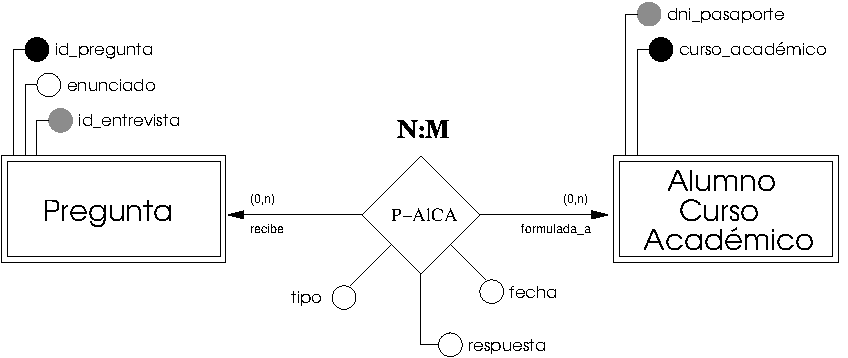
\includegraphics[]{07.Modelo_Entidad-Interrelacion/7.3.Analisis_Interrelaciones/diagramas/P-AlCA.pdf}
            \caption{Diagrama de la interrelación P-AlCA.}
            \label{diagramaP-AlCA}
            \end{center}
         \end{figure}

      \item[Descripción de los atributos] La interrelación presenta los
      siguientes atributos:

       \begin{itemize}
        \item \textbf{tipo}
          \begin{itemize}
            \item \textbf{Definición:} Establece el tipo de pregunta realizada,
            ya sea grupal o individual.
            \item \textbf{Dominio:} Unos de los valores: grupal o individual.
            \item \textbf{Carácter:} Obligatorio.
            \item \textbf{Ejemplo práctico:} individual.
            \item \textbf{Información adicional:} El dato \textbf{¿¿QUIÉN LO INTRODUCE??}.
         \end{itemize}
         \item \textbf{respuesta}
          \begin{itemize}
            \item \textbf{Definición:} Establece la contestación del alumno a la
            pregunta realizada.
            \item \textbf{Dominio:} Conjunto de caracteres alfanuméricos.
            \item \textbf{Carácter:} Obligatorio.
            \item \textbf{Ejemplo práctico:} Alto.
            \item \textbf{Información adicional:} El dato \textbf{¿¿QUIÉN LO INTRODUCE??}.
         \end{itemize}
          \item \textbf{fecha}
          \begin{itemize}
            \item \textbf{Definición:} Establece el día, mes y año cuando se
            formuló la pregunta.
            \item \textbf{Dominio:} Formato de fecha: dd/mm/aaaa.
            \item \textbf{Carácter:} Opcional.
            \item \textbf{Ejemplo práctico:} 01/01/2009.
            \item \textbf{Información adicional:} El dato \textbf{¿¿QUIÉN LO INTRODUCE??}.
         \end{itemize}
       \end{itemize}

      \item[Ejemplo práctico del tipo de interrelación]

      \item \begin{center}
            \begin{tabular}{ | r r | }
            \hline
            \multicolumn{2}{ | c | }{\textbf{Tipo de interrelación P-AlCA}} \\
            \hline
            \textbf{Pregunta} & \\
            id\_pregunta & 36 \\
            enunciado & Nivel de inglés \\
            id\_entrevista & 24 \\
            \hline
            \textbf{Alumno Curso Académico} & \\
            dni\_pasaporte & 01234567A \\
            curso\_académico & 2008 \\
            \hline
            \textbf{Atributos} & \\
            tipo & individual \\
            respuesta & Alto \\
            fecha & 01/01/2009 \\
            \hline
            \end{tabular}
         \end{center}
   \end{description}
